\documentclass{standalone}
\usepackage{tikz}
\begin{document}
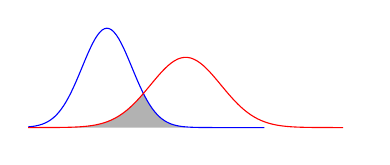
\begin{tikzpicture}
% define normal distribution function 'normaltwo'
\def\normaltwo{\x,{1/(sqrt(2*pi * .1)) *exp((-(\x-3)^2)/.2)}}
\def\normalone{\x,{1/(sqrt(2*pi * .2)) *exp((-(\x-4)^2)/.4)}}

% input y parameter
\def\y{4.4}

% this line calculates f(y)
\def\fy{4*1/exp(((\y-3)^2)/2)}

% Shade orange area underneath curve.
\fill [fill=gray!60] (2, 0) -- plot[domain=2:3.45, samples = 100,] (\normalone) -- plot[domain=3.45:4, samples = 10] (\normaltwo) -- (4,0) -- cycle;

% % Draw and label normal distribution function
\draw[color=blue,domain=2:5, samples = 100,] plot (\normaltwo) node[right] {};
\draw[color=red,domain=2:6, samples = 100,] plot (\normalone) node[right] {};

% % Add dashed line dropping down from normal.
% \draw[dashed] ({\y},{\fy}) -- ({\y},0) node[below] {$y$};

% % Optional: Add axis labels
% \draw (-.2,2.5) node[left] {$f_Y(u)$};
% \draw (3,-.5) node[below] {$u$};

% % Optional: Add axes
% \draw[->] (0,0) -- (6.2,0) node[right] {};
% \draw[->] (0,0) -- (0,5) node[above] {};

\end{tikzpicture}
\end{document}